\documentclass[tikz,border=10pt]{standalone}
\usepackage{tikz}
\usetikzlibrary{positioning}
\usetikzlibrary{shapes.geometric}% tikz node 形状的库
\usetikzlibrary{patterns}
\usepackage{tikz-feynman}
\begin{document}

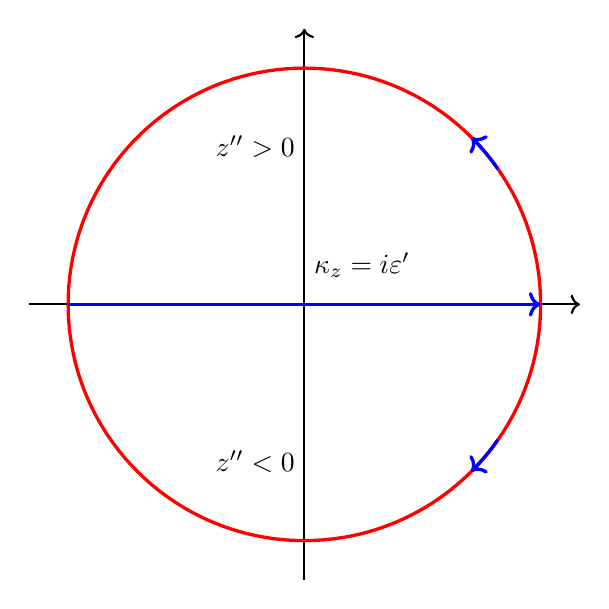
\begin{tikzpicture}
	\draw[thick,->] (-3.5,0)--(3.5,0);
	\draw[thick,->] (0,-3.5)--(0,3.5);
	\draw[red,very thick] (0,0) circle [radius=3cm];
	\draw[blue,very thick,->] (35:3) arc (35:45:3);
	\draw[blue,very thick,->] (-35:3) arc (-35:-45:3);
	\draw[blue,very thick,->] (-3,0)--(3,0);
	\node[anchor=west] at (0,.5) {$\kappa_z=i\varepsilon^{\prime}$};
	\node[anchor=east] at (0,2) {$z^{\prime\prime}>0$};
	\node[anchor=east] at (0,-2) {$z^{\prime\prime}<0$};
	\end{tikzpicture}

\end{document}